%%%%%%%%%%%%%%%%%%%%%%%%%%%%%%%%% Packages/Dokumentart %%%%%%%%%%%%%%%%%%%%%%%%%%%%%%%%%%%%%%%%%%%%%%%%%%%%%%%%%%%%%%%%%%%%%%%%%%%%%%%%%%%%%%%%%%%%%%%%%%%%%%%%%%%%%%%
\documentclass[ a4paper,	% Papierart
	%       10pt,		%
		11pt,		% Schriftgröße
	%	12pt,		%
		pdftex,		% PDF Umwandlung
	%	twoside		% 2-seitig
		] {report}	% Dokumenttyp Bericht

\usepackage[ngerman]{babel}	% Deutsches Sprachpaket/Silbentrennung etc.
\usepackage[utf8]{inputenc}	% verwendeter Codec (für Umlaute)
\usepackage[left=26mm,right=26mm,top=26mm,bottom=26mm]{geometry}
\usepackage{graphicx}		% für Bilder
\usepackage{cite}		% für bestimmte Zitierfunktionen
\usepackage{url}
\usepackage[footnote]{acronym}	% für Abkürzungen in Fußnote
\usepackage{caption}		% Um Bildunterschriften zu konfigurieren (mit, ohne erscheinen im Abkürzungsverzeichnis)
\usepackage{setspace}		% für Zeilenabstand

\onehalfspacing			% ab hier Zeilenabstand 1,5


%%%%%%%%%%%%%%%%%%%%%%%%%%%%%%%% Kopfzeile %%%%%%%%%%%%%%%%%%%%%%%%%%%%%%%%%%%%%%%%%%%%%%%%%%%%%%%%%%%%%%%%%%%%%%%%%%%%%%%%%%%%%%%%%%%%%%%%%%%%%%%%%%%%%%%%%%%%%%%%%%
\usepackage[automark]{scrpage2}			% Package für Kopfzeile	
\pagestyle{scrheadings} 			% Pagestyle
\automark[section]{chapter} 			% für Anzeigen des Unterkapitels (Standard Überkapitel)
\clearscrheadfoot \ihead{\headmark}		% ihead links, ohead rechts, chead mitte
\setheadsepline{0.4pt}				% Linie unter Kopfzeile
\cfoot[\pagemark]{\pagemark}			% Mitte Fußzeile Seitenzahl (selbe wie mit head (i,o,c))

%%%%%%%%%%%%%%%%%%%%%%%%%%%%%%%%%% Abkürzungen %%%%%%%%%%%%%%%%%%%%%%%%%%%%%%%%%%%%%%%%%%%%%%%%%%%%%%%%%%%%%%%%%%%%%%%%%%%%%%%%%%%%%%%%%%%%%%%%%%%%%%%%%%%%%%%%%%%%%%%
% Persöhnlich
\newcommand{\Autor}{Steffen Kurstak und Julian Kühn}
\newcommand{\MatrikelNummer}{Matrikelnummer}
\newcommand{\Kursbezeichnung}{TINF11B3}
%Firma
\newcommand{\dhLogo}{
\includegraphics[width=4cm]{Bilder/dhbw-logo.png}}
%Betreuer
\newcommand{\BetreuerDHBW}{Dr. Ralf Brune}
%Art der Arbeit
%\newcommand{\Was}{Praxisbericht}
%\newcommand{\WasErklaerung}{den vorliegenden \Was}
\newcommand{\Was}{Studienarbeit}
\newcommand{\WasErklaerung}{die vorliegende \Was}
%\newcommand{\Was}{Studienarbeit}
%\newcommand{\WasErklaerung}{die vorliegende \Was}
%\newcommand{\Was}{Bachelorarbeit}
%\newcommand{\WasErklaerung}{die vorliegende \Was}
%Deckblatt Infos
\newcommand{\Titel}{Analyse und Implementierung eines Honeypot-Systems}
\newcommand{\Dauer}{12 Wochen}
\newcommand{\Abschluss}{Bachelor of Engineering}
\newcommand{\Studiengang}{Informationstechnik}
\newcommand{\AbgabeDatum}{1. April 2013}

\begin{document}   %%%%%%%%%%%%%%%%%%%%%%%%%%%%%%%%%%%%%%%%%%%%%%%%%%%%%%%%%%%%%%%%%%%%%%%%%%%%%%%%%%%%%%%%%%%%%%%%%%%%%%%%%%%%%%%%%%%%%%%%%%%%%%%%%%%%%%%%%%%%%%%%%%%%

%%%%%%%%%%%%%%%%%%%%%%%%%%%%%%%%%% Titelseite %%%%%%%%%%%%%%%%%%%%%%%%%%%%%%%%%%%%%%%%%%%%%%%%%%%%%%%%%%%%%%%%%%%%%%%%%%%%%%%%%%%%%%%%%%%%%%%%%%%%%%%%%%%%%%%%%%%%%%%%%
\begin{singlespace}							% Zeilenabstand für Titelseite verringern
\begin{titlepage}
\begin{center}								% Referenzpunkt Seitenmitte
\vspace*{-2cm}								% 2 cm nach Links Platz lassen
\dhLogo\\[2cm]
{\Huge \Titel}\\[2cm]							% \Huge, \Large, \large sind versch. Schriftgrößen \bfseries ist Fett gedruckt
{\Huge\scshape \Was}\\[2cm]						% [] Inhalt ist Abstand zur nächsten Zeile
{\large f\"ur die Pr\"ufung zum}\\[0.5cm]
{\Large \Abschluss}\\[0.5cm]
{\large des Studienganges \Studiengang}\\[0.5cm]
{\large an der}\\[0.5cm]
{\large Dualen Hochschule Baden-W\"urttemberg Karlsruhe}\\[0.5cm]
{\large von}\\[0.5cm]
{\large\bfseries \Autor}\\[1cm]
{\large Abgabedatum \AbgabeDatum}
\vfill									% ermöglicht es unterhalb der Seitengrenze zu schreiben
\end{center}								% Referenzpunkt Mitte beenden

\begin{tabular}{l@{\hspace{2cm}}l}					% Beginn Tabelle mit einer Spalte nach der 2cm Platz gelassen wird bevor die nächste beginnt
Bearbeitungszeitraum	         & \Dauer 			\\
Matrikelnummer	                 & \MatrikelNummer		\\
Kurs			         & \Kursbezeichnung		\\
Gutachter der Studienakademie	 & \BetreuerDHBW		\\
\end{tabular}								% Tabelle abschließen
\end{titlepage}
\end{singlespace}								% Titelseite abschließen
%%%%%%%%%%%%%%%%%%%%%%%%%%%%%%%%%%%%%%%%%%%%%%%%%%%%%%%%%%%%%%%%%%%%%%%%%%%%%%%%%%%%%%%%%%%%%%%%%%%%%%%%%%%%%%%%%%%%%%%%%%%%%%%%%%%%%%%%%%%%%%%%%%%%%%%%%%%%%%%%%%%%%%%%

%Erklärung
%%%%%%%%%%%%%%%%%%%%%%%%%%%%%%%%%%%%%% Erklaerung %%%%%%%%%%%%%%%%%%%%%%%%%%%%%

\newpage
\thispagestyle{empty}

\begin{center}
\Large\bfseries Erkl\"arung
\end{center}

\noindent
Gem\"a\ss{} \S16 (3) der "`Studien- und Pr\"ufungsordnung f\"ur den Studienbereich
Technik"' vom 1.11.2007.

\medskip
\noindent
Ich habe \WasErklaerung\ selbstst\"andig verfasst und
keine anderen als die angegebenen Quellen und Hilfsmittel verwendet.

\vspace{3cm}
\noindent
\underline{\hspace{4cm}}\hfill\underline{\hspace{6cm}}\\
Ort~~~~~Datum\hfill Unterschrift\hspace{4cm}


%%%%%%%%%%%%%%%%%%%%%%%%%%%%%%%%%%%%%% Kurzzusammenfassung %%%%%%%%%%%%%%%%%%%%%%%%%%%%%%%%%%%%%%%%%%%%%%%%%%%%%%%%%%%%%%%%%%%%%%%%%%%%%%%%%%%%%%%%%%%%%%%%%%%%%%%%%%%%%
\begin{abstract}
\begin{onehalfspace}

Hier steht eine Kurzzusammenfassung.

\end{onehalfspace}
\end{abstract} %%%%%%%%%%%%%%%%%%%%%%%%%%%%%%%%%%%%%%%%%%%%%%%%%%%%%%%%%%%%%%%%%%%%%%%%%%%%%%%%%%%%%%%%%%%%%%%%%%%%%%%%%%%%%%%%%%%%%%%%%%%%%%%%%%%%%%%%%%%%%%%%%%%%%%%%%%


%%%%%%%%%%%%%%%%%%%%%%%%%%%%%%%%%% Verzeichnisse %%%%%%%%%%%%%%%%%%%%%%%%%%%%%%%%%%%%%%%%%%%%%%%%%%%%%%%%%%%%%%%%%%%%%%%%%%%%%%%%%%%%%%%%%%%%%%%%%%%%%%%%%%%%%%%%%%%%%%%%
\chapter*{Sperrvermerk}
Die vorliegende Arbeit beinhaltet interne vertrauliche Informationen 
der z.B. Firma EDEKA Handelsgesellschaft Südwest mbH.\\ 

\noindent Die Weitergabe des Inhaltes der Arbeit und eventuell beiliegender Zeichnungen und Daten im Gesamten oder in Teilen ist grundsätzlich untersagt.\\ 

\noindent Es dürfen keinerlei Kopien oder Abschriften – auch in digitaler Form - gefertigt werden. Ausnahmen bedürfen der schriftlichen Genehmigung der Firma EDEKA Handelsgesellschaft Südwest mbH in Abstimmung mit dem/der Verfasser/in.\\

\noindent Die vorliegende Arbeit ist nur den Korrektoren sowie ggf. den Mitgliedern des Prüfungsausschusses zugänglich zu machen. \\

\vspace*{2cm}
\noindent(Stempel)
\vspace*{1.5cm}\newline
\noindent(Ort, Datum)
\vspace*{1cm}\newline
\noindent(Unterschrift des Betreuers bzw. Ausbildungsleiters)


\begin{singlespace}			 % Zeilenabstand für Verzeichnisse 1	
\tableofcontents 			 % Inhaltsverzeichnis
\listoffigures	 			 % Abbildungsverzeichnis
\listoftables				 % Tabellenverzeichnis
\end{singlespace}	 		 % Zeilenabstand wieder ausstellen
%\listofequations			 % Formelverzeichnis
%\listoflistings 			 % Listenverzeichnis
\chapter*{Abkürzungsverzeichnis}		  % das * verhindert das das Kapitel eine Nummerierung erhält
\begin{singlespace}				  % Einfacher Zeilenabstand wegen Platz

\begin{acronym}[wwwwwwwwwwwwwwwww]                % Inhalt der eckigen Klammer ist der Abstand von der Abkürzung zur Erklärung/ Beginn der Acro Umgebung
	\setlength{\itemsep}{-\parsep}		  % Veringert den Abstand untereinander
	\acro{Abk.}{Vollständige Abkuerzung}

\end{acronym}					  % Ende der Acro Umgebung

\end{singlespace}
 %Abkuerzungsverzeichnis
\newpage %%%%%%%%%%%%%%%%%%%%%%%%%%%%%%%%%%%%%%%%%%%%%%%%%%%%%%%%%%%%%%%%%%%%%%%%%%%%%%%%%%%%%%%%%%%%%%%%%%%%%%%%%%%%%%%%%%%%%%%%%%%%%%%%%%%%%%%%%%%%%%%%%%%%%%%%%%%%%%%%%

%%%%%%%%%%%%%%%%%%%%%%%%%%%%%%%%%% Kapitel einbinden %%%%%%%%%%%%%%%%%%%%%%%%%%%%%%%%%%%%%%%%%%%%%%%%%%%%%%%%%%%%%%%%%%%%%%%%%%%%%%%%%%%%%%%%%%%%%%%%%%%%%%%%%%%%%%%%%%%%%
\chapter{Einleitung}			% Kapitelname

\section{Ziele der Arbeit}
Im Rahmen dieser Arbeit soll ein Honeypot implementiert werden und über das Internet als potentielles Angriffsziel für Hacker dienen. Anschließend sollen die Angriffe ausgewertet und diverse Statistiken erstellt werden. Zudem sollen ein oder zwei Angriffe, mit Hilfe von Tools, detailliert aufgearbeitet werden. Für die Implementierung des Honeypots ist auch ein Softwarevergleich nötig, um eine passende Software zu finden. Möglich ist auch der Einsatz eines kommerziellen Honeypots.
Für die Analyse der Angriffe ist ebenfalls der Einsatz mehrere Tools möglich und erwünscht. 			% Einbinden der Unterkapitel
\section{Ziele der Arbeit}
\section{Stand der Technik}
Zwischen 2000 und 2006 war der Honeypot am populärsten. Neben Firmen haben auch Privatnutzer mit Hilfe der Honeypots angefangen Hacker zu studieren. Da ein Honeypot allerdings gerade in der Industrie nur Geld kostet und oftmals keinen messbaren Mehrwert bringt, ist der Einsatz von Honeypots zurückgegangen. Zudem sind auch die Communitys zurückgegangen und der damit einhergehend Support von OpenSource Projekten. Die Honeyport-Software Honeyd ist hierfür ein passendes Beispiel, da das letzte Release der Software bereits aus dem Jahre 2007 ist. Somit ist bei dem Einsatz von OpenSource Produkten in dieser Studienarbeit, mit Problemen bezüglich Dokumentation und Support zu rechnen. Hilfreich wäre hier eine kommerzielle Lösung, um diesen Problemen aus dem Weg zu gehen. 
\section{Umgebung der Arbeit}
Die Studienarbeit \glqq Analyse und Implementierung eines Honeypots-Systems\grqq wird im Rahmen des Bachelor Studiengangs Informationstechnik an der DHBW-Karlsruhe durchgeführt. Ausgearbeitet wird das Thema von den Studenten Julian Kühn und Steffen Kurstak. Für die Durchführung dieser Arbeit steht ein Server mit zwei Netzwerk-Ports zur Verfügung sowie zwei öffentliche IP-Adressen der DHBW-Karlsruhe. Das Betriebssystem des Servers wird voraussichtlich auf Linux basieren.

Neben dem Server wird auch der kauf eines vorinstallierten Honeypots angestrebt, welcher damit ebenfalls zur Verfügung stehen wird

Die Dokumentation dieser Arbeit wird in \LaTeX geschrieben. Für einen vereinfachten Umgang mit \LaTeX wird die Software TeXstudio eingesetzt. Ein ausschlaggebendes Kriterium für den Einsatz von \LaTeX, ist der unkomplizierte Umgang bei einem parallelen Arbeiten der Autoren. Durch die Untergliederung in einzelne Dateien werden Konflikte vermieden. Mit Hilfe des Repositorys GitHub wird die Versionsverwaltung vorgenommen. 
\newpage

\chapter{Honeypots}			% Kapitelname


\section{Definition}

Einleitend und noch oberflächlich erklärt ist die Aufgabe eines Honeypots, einen Angreifer von einem bedeutsamen Ziel abzulenken. In der Informationstechnik erfüllen Honeypots, je nach Einsatzgebiet und Ansicht des Entwicklers, verschiedene Aufgaben.

Einige Unternehmen sehen den Einsatz eines Honeypots als ein Intrusion Detection System. Für andere ist es nur eine Täuschung für Hacker, welche dadurch von den produktiven Systemen abgelenkt werden sollen. Ein weiterer Nutzen eines Honeypots ist es, die angreifenden Hacker analysieren zu können und somit neue Vorgehensweisen und Trends der Hacker zu erkennen. Diese Informationen sind vor allem für Sicherheitsfirmen relevant, da sie dabei neue Viren, Trojaner oder weitere Schadsoftware erkennen können.

Trotz dieser verschiedenen Einsatzmöglichkeiten hat Lance Spitzner eine passende Definition gefunden: \glqq A honeypot is security resource whose value lies in being probed, attacked, or compromised.\grqq \cite{spitzner.2002a}

Der Honeypot ist nach Spitzner eine Sicherheits-Ressource deren Wert darin liegt, erforscht, attackiert und kompromittiert zu werden. Durch diese Definition ist offen gelassen, welchen Nutzen der Anwender daraus zieht. Mit dieser allgemein gehaltenen Definitionen können nun Ziele eines Honeypots im nächsten Kapitel beschrieben werden.
			% Einbinden der Unterkapitel
\section{Ziele}

Die Ziele eines Honeypots lassen sich in zwei Kategorien einteilen. Das sind zum einen die \glqq Research Honeypots\grqq und zum anderen die \glqq Production Honeypots\grqq. 

Die unterschiedlichen Ziele dieser Honeypots werden in den folgenden Kapiteln beschrieben.

\subsection{Research}

Ein Research Honeypot wird für die Untersuchung und Forschung der Angriffe eingesetzt. Der Honeypot wird meist getrennt von allen Produktivsystemen aufgebaut. In Abb. \ref{hnet:reHon1} wird der Honeypot vor die Firewall des Produktivnetzes installiert. Dadurch wird versucht mögliche Angreifer weit weg von dem Produktiv-Systemen zu halten. 
\\
\begin{figure}[ht]
    \centering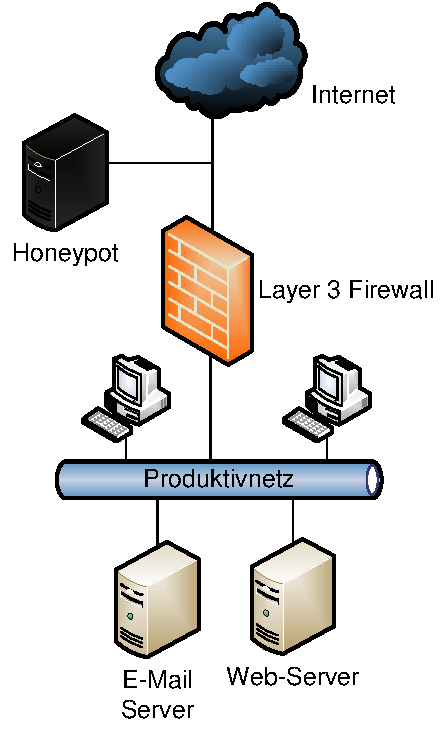
\includegraphics[scale=0.6]{Bilder/Research_1.pdf}
  \caption{Research Honeypot - Variante I}
  \label{hnet:reHon1}
\end{figure}


Eine weitere Möglichkeit eines solchen Aufbaus ist in Abb. \ref{hnet:reHon2} dargestellt. Hier wird der Honeypot durch die Layer 3 Firewall von dem Produktivnetz getrennt. Bei diesem Aufbau muss genau auf die Firewall-Einstellungen geachtet werden, um den Angreifern nicht ungewollt einen Sprungserver zu den produktiven Systemen zur Verfügung zu stellen.

\begin{figure}[ht]
  \centering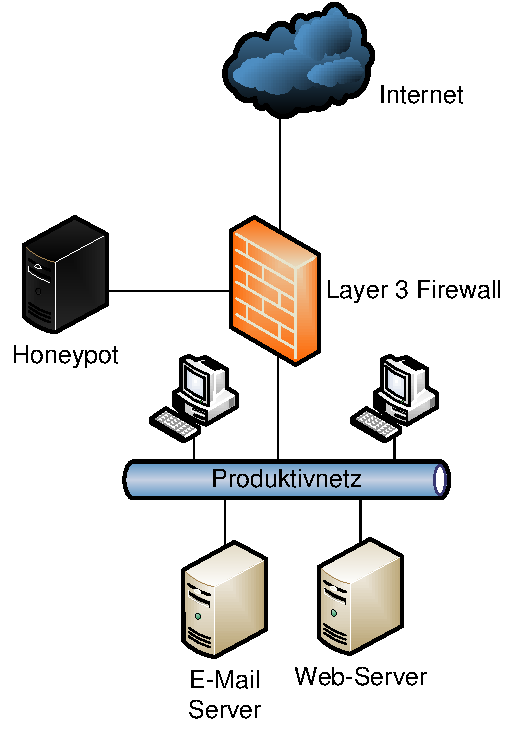
\includegraphics[scale=0.6]{Bilder/Research_2.pdf}
  \caption{Research Honeypot - Variante II}
  \label{hnet:reHon2}
\end{figure}
Es geht hier primär um die Erkennung von neuen Würmern, Trojanern und weiterer Schadsoftware. Neben der Schadsoftware werden auch Angriffe von Hackern sowie der nicht so qualifizierten \glqq Skript-Kiddies\grqq untersucht.

Bei jedem Angriff werden Daten und Informationen über den Angreifer gesammelt. Dabei lässt sich häufig ermitteln wer, womit und evtl. auch warum er angegriffen hat. Setzt man mehrere Honeypots an verschiedenen Standorten ein, lassen sich mit den gesammelten Daten neue Trends der Angreifer erkennen. Durch diese Informationen versuchen Unternehmen Angriffe auch vorhersagen zu können und die Vorgehensweise der Angreifer besser zu verstehen. Mit den gesammelten Daten können auch neue Tools, mit denen vorallem Skript-Kiddies arbeiten, aufgedeckt werden.

Um die Daten besser auswerten zu können teilen verschiedene Organisationen ihre gesammelten Daten und Erkenntnisse mit anderen Unternehmen. Die große Anzahl der Daten ermöglicht eine bessere Analyse sowie eine genauere Trend-Erkennung. 

Research Honeypots dienen somit nicht direkt zur Risiko-Minimierung. Vielmehr helfen die Erkenntnisse, die Angriffs-Prävention und Erkennung zu verbessern.			%
\subsection{Production}

Im Gegensatz zu einem Research Honeypot wird ein Production Honeypot, wie der Name schon sagt, in einem produktiven Umfeld eingesetzt. 
\\
\begin{figure}[ht]
    \centering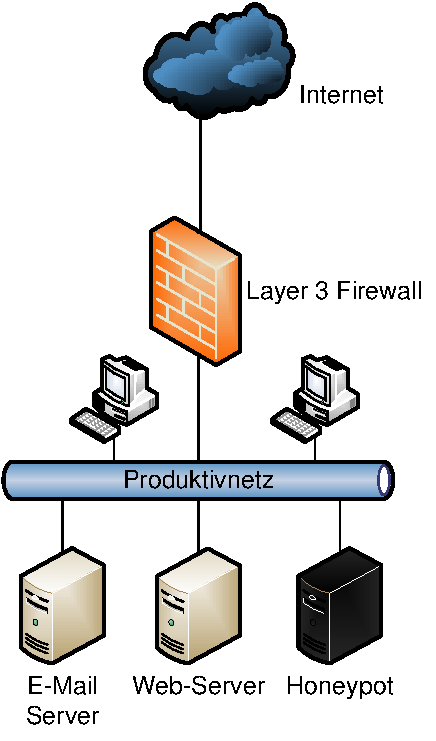
\includegraphics[scale=0.6]{Bilder/produktiv.pdf}
  \caption{Research Honeypot}
  \label{hnet:geni}
\end{figure}
\\
\begin{itemize}							% Beginn der Aufzählungsumgebung
\item{\textbf{Prevention}} \\ asdasda sfs				
\item{\textbf{Detection}} \\
\item{\textbf{Response}} \\
\end{itemize}			%			%
\section{Rechtliche Grundlage}

Der Betreiber eines Honeypots stellt bewusst ein Angriffsziel für blackhats zur Verfügung. Nutzt ein blackhat den Zugriff auf einen Honeypot, um von dort aus weitere Straftaten zu begehen, kommen dabei auch Rechtliche Fragen auf. Kann dem  Betreiber des Honeypots fahrlässiges handeln oder gar eine Beihilfe vorgeworfen werden?

Hinzu kommt die Frage, mit der sich auch schon \cite{dornseif.2012a} beschäftigt hat, dürfen die Daten der blackhats verwendet werden, ohne das Wissen gerade an einem Experiment teil zu nehmen? 

In den folgenden Kapiteln werden diese Fragestellungen kurz beleuchtet. 

\subsection{Zivil- und Strafrecht}
Sollte der Honeypot, von einem blackhat, für einen Übergriff auf einen unbeteiligten Dritten genutzt werden, könnte ihm Strafrechtlich eine Beihilfe vorgeworfen werden. Um eine Beihilfe einer Straftat zu leisten, erklärt \cite{dornseif.2012a}, muss eine aktive Hilfeleistung seitens des Honeypts-Betreibers nachgewiesen werden.

Im Fall der Honeypots ist dieser Nachweis nicht möglich, da es gezielt Maßnahmen zum Schutz vor Übergriffen durch den Honeypot auf fremde Systeme gibt. Der Sicherheitsstandard eines Honeypots ist oft nicht geringer als der anderer Systeme. Zudem kann auch nicht behauptet werden, dass sich ein Honeypot einem blackhat explizit aufdrängt oder ihn zu einer Straftat verleitet.

Zivilrechtlich stellt sich nun die Frage, ob der Betreiber für einen aufgekommen Schaden Haftbar gemacht werden kann. \cite{dornseif.2012a} beantwortet diese Frage ebenfalls mit nein. Um den Betreiber Haftbar zu machen, muss der Honeypot aktiv anderen Systemen schaden zufügen. Da ein solcher Sachverhalt nicht vorliegt, bleibt die Möglichkeit einer Unterlassung der Absicherung. Diese Anschuldigung stützt sich auf der sogenannten Verkehrssicherungspflicht. Hierbei geht es im groben darum, dass der Betreiber die Gefahren, die bewusst durch den Honeypot geschaffen werden, mit angemessenen Vorkehrungen gering hält. Somit soll der schaden Dritter vermieden werden.

Auch hier ist zu sagen, dass Honeypots ausreichend überwacht und gesichert werden, wodurch eine Unterlassung der Absicherung ausgeschlossen werden kann.
\subsection{Datenschutz}
Ist ein Angreifer auf einem Honeypot zu Gange, wird er oftmals von Tools überwacht und aufgezeichnet. Diese Aufzeichnungen stehen dem Betreiber zur Verfügung und dass ohne das Wissen des Angreifers. Dornseif zweifelt dabei die Unwissenheit des Angreifers an und argumentiert damit, dass die blackhat-Community über die Existenz von Honeypots informiert sind. Somit nehmen sie bei ihren Angriffen eine Aufzeichnung und Überwachung in Kauf. 

Hinzu kommt, dass bei den Angriffen von blackhats keine personenbezogenen Daten in die Hände des Betreibers fallen. Mit dieser Argumentation kann auch der Datenschutzrechtliche Hintergrund entkräftet werden.	


\newpage

\chapter{Honeynets}
Honeynets bestehen aus mehreren virtuellen oder physikalischen Honeypots, die ein komplettes Netzwerk darstellen. Jede Netzwerkkomponente und jeder Server kann dabei als Honeypot angesehen werden. So besteht die Möglichkeit ein komplettes Produktivnetz nachzustellen, welches dem Hacker den Eindruck vermittelt, in ein produktiv verwendetes Firmennetz eingedrungen zu sein.\cite{grimes.2005a}

\section{Anforderungen eines Honeynets}
\noindent Um ein effektives Honeynet zu erstellen, müssen verschiedenen Anforderungen erfüllt werden. Diese Anforderungen können Honeynets grob ich drei Kategorien unterteilt werden\cite{spitzner.2002a}:\\

\noindent\textbf{Data Control: }\\
Datenkontrolle bedeutet, dass der Betreiber eines Honeypots oder Honeynets die Kontrolle der ein- und ausgehenden Datenpakete behält. Gelingt es dem Hacker dem Honeynetbetreiber diese Kontrolle zu entreißen, besteht die Möglichkeit, dass der Hacker einen Angriff auf das Produktivnetz oder über das Internet startet. Da es sich bei der Datenkontrolle um ein großes Sicherheitsrisiko handelt sollte versucht werden folgende Punkte einzuhalten\cite{spitzner.2002a}:
\begin{itemize}
\item Datenkontrolle sollte automatisiert, jedoch auch manuell stattfinden
\item Die Datenkontrolle sollte mindestens durch zwei Schichten kontrolliert werden (falls eine Anwendung nicht erfolgreich sein sollte)
\item Alle ein- und ausgehenden Verbindungen sollten kontrollierbar bleiben
\item Jede unautorisierte Aktion soll kontrollierbar sein, ein anderes System im Produktivnetz darf nicht angreifbar sein
\item Die Datenkontrolle muss jederzeit durch den Administrator konfigurierbar sein
\item Verbindungen sollen für den Angreifer so schwer wie möglich erkannt werden
\item Mindestens zwei Benachrichtungsmöglichkeiten bei Aktivitäten im Honeynet
\item Auf die Datenkontrolle muss über einen Remote-Zugriff zugegriffen werden können
\end{itemize}
\noindent Die Datenkontrolle muss für den Angreifer unsichtbar sein. Zu strenge Sicherheitsvorkehrungen können den Hacker jedoch verunsichern und ihn auf den Honeypot aufmerksam machen (z.B. ausgehende Verbindungen blockieren). Jedoch kann z.B. eine Limitierung der ausgehenden Verbindungen ein gutes Mittel gegen den Verlust den Datenkontrolle sein\cite{WebHnet.2006b}\cite{spitzner.2002a}. \\

\noindent\textbf{Data Capture: }\\
\noindent Die Informationen, die ein Hacker während eines Angriffes hinterlässt, müssen möglichst reichhaltig und unauffällig dokumentiert werden. Für die Datensammlung gibt es verschiedene Möglichkeiten die Aktionen eine Hackers aufzuzeichnen\cite{grimes.2003a}.
\begin{itemize}
\item Packet Sniffing: Zum aufzeichnen des kompletten Netzverkehrs (ein- und ausgehende Pakete).
\item Keystroke Logging: Das aufzeichnen der vom Hacker ausgeführten Tastenanschläge.
\item Snapshot Software: Vergleicht Betriebssystemkonfigurationen vor- und nach der Kompromittierung und hält die Änderungen fest.
\item Log-Dateien wie z.B. Log-Daten eines Netzwerkgerätes wie Switch und Router
\end{itemize} 
Wichtig bei diesen Programmen ist es, dass sie für den Hacker nicht ersichtlich sein dürfen. Findet der Angreifer eines dieser Programme ist dieser alarmiert und wird die Flucht ergreifen\cite{spitzner.2002a}.
Das Honeynet-Project definiert eine effektive Datenanalyse wie folgt:\cite{spitzner.2002a}
\begin{itemize}
\item Keine aufgezeichneten Honeypot-Daten dürfen lokal auf diesen gespeichert werden (diese könnten vom Angreifer erkannt und modifiziert werden). Als Honeypot-Daten zählen alle Daten die bezüglich des Honeypots und dessen Umgebung aufgezeichnet werden.
\item Folgende Aktivitäten müssen ein Jahr lang aufgezeichnet werden: Netzwerkaktivitäten, Systemaktivitäten, Anwendungsaktivitäten und Benutzeraktivitäten.
\item Der Honeypot oder Honeynet Administrator muss jederzeit ortsunabhängig auf aufgezeichnete Daten Zugreifen können.
\item Aufgezeichnete Daten müssen für zukünftige Analysen automatisch archiviert werden.
\item Für jeden aktive Honeypot muss eine standardisierte Log-Datei existieren.
\item Für jeden kompromittierten Honeypot muss ein standardisierte Log-Datei existieren.
\item Alle gesammelten Daten müssen die GMT Zeitzone verwenden. Daten können zwar mit der lokalen Zeitzone aufgezeichnet werden, müssen jedoch für eine Analyse in das GMT Zeitformat konvertiert werden.
\item Anwendungen, die zur Aufzeichnung von Aktivitäten dienen, müssen sicher gegen Modifikationen sein, um die Integrität der aufgezeichneten Daten sicherzustellen.
\end{itemize}

\noindent\textbf{Data Collection: }\\
\noindent Bei einem verteilten System wie z.B. bei einem Honeynet muss es eine zentrale Stelle geben, in der die Informationen gesammelt und gespeichert werden. Daten werden nie direkt auf einem Honeypot protokolliert, sondern an ein zentrales System übertragen. Wichtig hierbei ist es, dass die Daten sicher und unverändert an das System übertragen werden. Der Angreifer soll nicht die Möglichkeit haben einen Angriff zu vertuschen, oder gar das System selbst anzugreifen\cite{WebHnet.2006b}. Die Anforderungen an die Datensammlung kann in vier Elemente unterteilt werden\cite{spitzner.2002a}:
\begin{itemize}
\item Jeder Honeypot im Honeynet soll in der Sammlung identifizierbar sein. Dies kann z.B. durch eine Art \acf{IP/DNS} gemappte Datenbank erreicht werden.
\item Die Daten müssen vom Honeypot sicher auf das Sammelnde System übertragen werden. Die Integrität der Daten darf nicht während der Übertragung verändert werden können.
\item Eine Möglichkeit zur Anonymisierung der Daten. 
\item Eine Standardisiertes \acf{NTP}, um sicherzustellen dass alle Daten richtig synchronisiert wurden.
\end{itemize}

\noindent\textbf{Data Analysis: }\\
\noindent Die gewonnenen Informationen müssen dem Zweck entsprechend ausgewertet werden. Je nach Ziel des Honeypots müssen z.B. Gegenmaßnahmen getroffen, oder aus dem gelernten Wissen Schlüsse gezogen werden, um in Zukunft eine Kompromittierung eines Produktivsystems zu verhindern\cite{WebHnet.2006b}.

\section{Architektur eines Honeynets}
Es gibt zwei verschieden Arten von Architekturen die sich im Laufe der Zeit durchgesetzt haben. Diese werden in Generation I und Generation II Honeynets (Abk. GenI und GenII) unterteilt.\\
\subsection{GenI Honeynet}
Bei einem GenI Honeynet wird das gesamte Netz durch eine Firewall in drei Teile unterteilt. Der erste Teil ist das Produktivnetz indem sich das zentrale Management System befindet. Der zweite Teil ist das Internet, welcher das Zugangsmedium des Angreifers darstellt. Der dritte und letzte Teil ist das Honeynet\cite{WebGenI.2006b}. 

GenI Honeynets gelten als die ersten richtigen High-Interactive Honeypots, da sie weit mehr Informationen als normale Honeypot, und unbekannte Angriffe aufzeichnen können\cite{spitzner.2002a}.

Der Prozess der Datensammlung beginnt bereits mit passieren der Firewall. Dort können Informationen wie die verwendeten Protokolle, Zeitstempel,IP-Adressen und Ports gesammelt werden. Außerdem wird hier kontrolliert wie oft der Angreifer eine Verbindung eingehen kann (Data Control). Wie viele Versuche zugelassen werden hängt vom Verwendungszweck des Honeynets ab. Der Router zwischen Honeynet und Firewall unterstützt diese auf zwei verschiedene weisen. Zum Einem versteckt er die Firewall vor dem Hacker. Der Angreifer denkt, er greift auf einen produktiven Router zu. Zum Anderen unterstützt er die Firewall in Sachen Zugriffskontrolle. So kann ein Single-Point-of-Failure vermieden werden\cite{grimes.2003a}\cite{WebGenI.2006b}. 

Ein \acf{IDS}-System steht nun noch zwischen dem Angreifer und den Honeypots. Dieses ist meist über einen Switch (oder wie in Abb. \ref{hnet:geni} mit einem Router) mit dem gesamten Honeynet verbunden. Dort werden alle Netzwerkaktivitäten protokolliert und bei bestimmten Angriffsmustern gegebenenfalls ein Alarm ausgelöst\cite{spitzner.2002a}. 

\begin{figure}[ht]
    \centering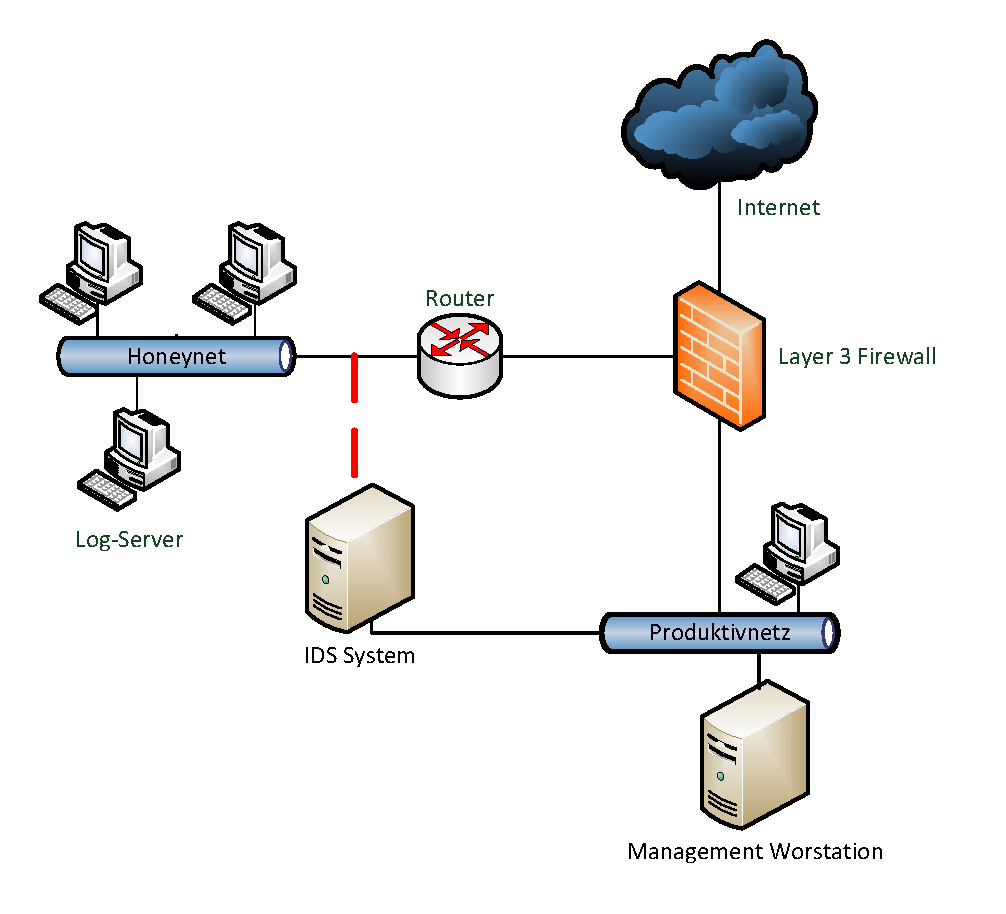
\includegraphics[scale=0.5]{Bilder/GenI.pdf}
  \caption{GenI Honeynet}
  \label{hnet:geni}
\end{figure}

\noindent Die GenI Technologie bietet sich besonders an, um automatisierte oder Anfänger-Hacks zu erkennen. Meist handelt es sich dabei um Ziele, deren Schwachstelle zufällig entdeckt wird, und es dadurch zu einem Angriff kommt. 
Die Architektur ist nicht effektiv für fortgeschrittene Angreifer, oder Hacker, die ein bestimmtes System angreifen wollen. Zum einen sind diese relativ einfach über einen Fingerprint ausfindig zu machen, zum Anderen bestehen sie meist aus einer Standardinstallation eines Betriebssystems, weswegen sie für Angreifer meist uninteressant wirken\cite{spitzner.2002a}.\\

\noindent\textbf{Methoden zur Datenkontrolle}\\
\noindent Die Datenkontrolle eines GenI Honeypots besteht im Grunde aus der Layer 3 Firewall, die das Produktivnetz vom Honeynet trennt. Die Firewall erlaubt jeglichen Zugriff in das Netz, limitiert jedoch die ausgehenden Verbindungen (nicht Pakete). Der Firewall wird vom Administrator eine Grenze für ausgehende Verbindungen mitgeteilt, nach erreichen dieser wird jeder ausgehender Verbindungsversuch geblockt. Je mehr Verbindungen erlaubt sind, desto mehr Freiheiten hat der Hacker seine Aktionen durchzuführen. Um den Schaden zu minimieren die der Hacker verursacht, kann auch eine geringe Grenze gewählt werden. Automatisierte Attacken können so z.B. weiterhin festgestellt werden. Das Honeynet Project empfiehlt hierfür die Linux Firewall IPTables oder als kommerzielle Version FireWall-1 \cite{spitzner.2002a}.\\

\noindent\textbf{Methoden zur Datenaufzeichnung}\\
\noindent Die Datenaufzeichnung eines GenI Honeynets muss, wie zuvor definiert (vgl. Kapitel 3.1), für den Angreifer unsichtbar sein. Die Daten, die gesammelt werden, dürfen nicht lokal auf dem Honeypot gespeichert werden. Um dies zu verwirklichen werden die Daten in verschiedenen Schichten.
Die erste Schicht ist die Logging-Aktivität auf der Firewall. Alle Daten, die in das Honeynet gelange, müssen zunächst durch die Firewall. Dort können zwar keine Informationen wie Tastendrücke oder Packet-Payloads aufgezeichnet werden, jedoch können Protokoll Header, in denen sich Informationen wie Zeitpunkt, Quell- und Zieladresse sowie Quell- und Zielport befinden, ausgelesen und aufgezeichnet werden\cite{spitzner.2002a}. 

Die zweite Schicht ist das IDS-System, welches mit dem Produktivnetz und dem Honeynet jeweils mit einem Interface verbunden ist. Das Interface, dass mit dem Honeynet verbunden ist besitzt keine IP-Adresse. Es gilt als passives Interface (rote Linie in Abb. \ref{hnet:geni}), welches den kompletten Datenverkehr des Honeynets aufzeichnet, jedoch keine Angriffsfläche für den Hacker bietet, da es keine IP-Adresse besitzt. Das zweite Interface erlaubt es dem Administrator im Produktivnetz auf die gesammelten Daten zuzugreifen. Das IDS zeichnet die kompletten Datenpakete mit Payload auf und stellt diese später für eine Datenanalyse zur Verfügung. Die zweite Aufgabe des IDS ist es, eine Warnung bei ungewöhnlichen Aktivitäten zu geben.

Die dritte Schicht stellen die Honeypots selbst dar. Alle System und 
\subsection{GenII und GenIII Honeynets}
Die zweite Generation von Honeynets verwendet ein Gateway, welches die Funktionen der in GenI verwendetet Komponenten enthält, und diese noch weiter ergänzt. Dieses Gateway (meist Honeywall genannt) besteht nicht wie in GenI aus einem Layer-3 Router sondern aus einer Layer-2 Bridge. Dies verhindert z.B. dass der Angreifer über die TTL-Zähler eines IP-Paketes dn Router erkennen würde. Alle zuvor genannten Anforderungen werden in der Honeywall erfüllt. Für die Datenkontrolle werden hier wie in GenI die Verbindungen limitiert (oft mit dem Programm IPTables), um so DOS-Angriffe zu vermeiden und die Kontrolle über die Verbindungen zu erhalten. Zusätzlich bietet sich nun auch die Möglichkeit Zugriffe die über bestimmte Protokolle einzeln zu limitieren.

Ein IDS oder IPS verhindert weiterhin das der Hacker vom Honeynet aus einen Angriff auf das Produktivsystem oder in das Internet starten kann. Die Zugriffskontrolle und das IDS sammeln wie beim GenI Honeypot die Daten. In Abb. \ref{hnet:genii} befindet sich ein Beispiel einer GenII Honeynet Architektur.
\\
\begin{figure}[]
    \centering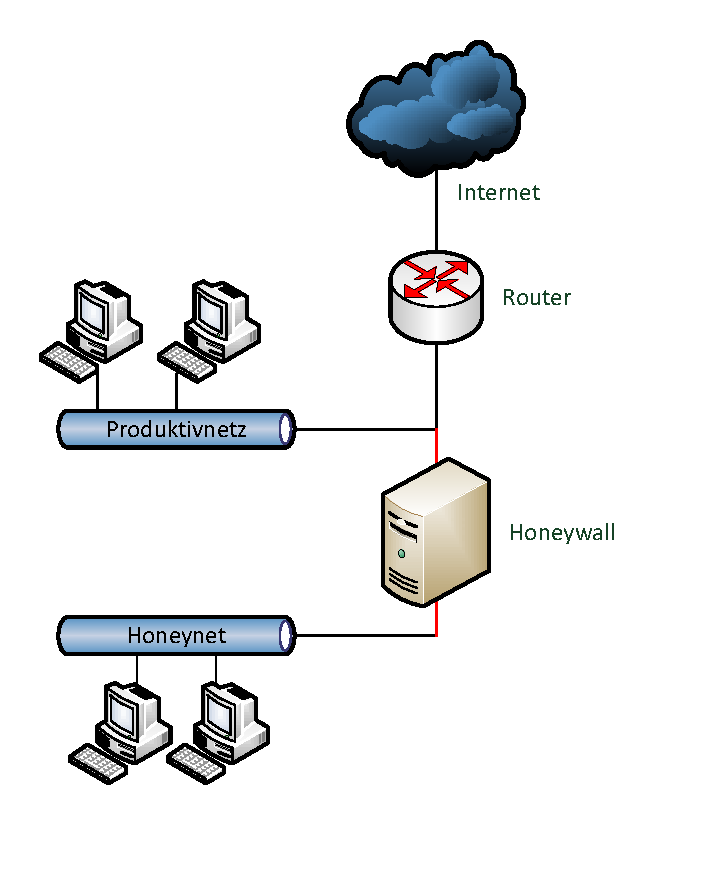
\includegraphics[scale=0.5]{Bilder/GenII.pdf}
  \caption{GenII Honeynet}
  \label{hnet:genii}
\end{figure}
\\
\noindent Ende 2004 wurde die vorerst letzte Generation von Honeynets vorgestellt. Ein GenIII Honeynet besitzt die selbe Netzwerkarchitektur wie dessen Vorgänger, behebt jedoch einig dessen Schwachstellen. Bei dem Versuch einen Honeynet Standard und eine Möglichkeit zu finden, ein Honeynet leichter zu Erstellen, veröffentlichte das Honeynet-Project (www.honeynet-project.org) eine CD, die alle Anforderungen eines Honeynets beinhaltet. Diese CD (\emph{Roo} genannt) wird als dritte Generation angesehen. Die aktuelle Version (1.4, Stand: 2014) bietet neben der verbesserten Datensammlung ,eine grafische Web-Oberfläche zur Datenanalyse, und unterstützt weiter Tools wie Sebek und Hflow2 (Siehe Kapitel Tools).


\newpage

\chapter{Implementierungsarten}
Wie viele Informationen ein Honeypot sammeln kann, hängt von seine Implementierungsart ab. Je nach Zweck und Aufwand kann zwischen den in diesem Kapitel genannten Arten unterschieden werden.

\section{Typen von Honeypots}
Die Funktionsweise von Honeypots ist von der Implementierungsart abhängig. Dabei spielt der gewünschte Grad der Interaktion, sowie der Zweck des Honeypots eine Rolle (Research oder Production). Je nach Anwendungsgebiet wird die dafür nützlichste Implementierung verwendet. Grundlegend wird dabei zwischen folgenden Implementierungsmöglichkeiten unterschieden:\\

\renewcommand{\arraystretch}{1.5}
\begin{table}[h]
\caption{Interaktionsgrade mit den zugehörigen Eigenschaften\cite{spitzner.2002a}}
\label{interTab}
\begin{center}
\begin{tabular}{|c|c|c|c|c|}\hline
   \textbf{Interaktions-} & \textbf{Installation und} & \textbf{Aufstellung und} & \textbf{Informations-} & \textbf{Risiko}\\ 
   \textbf{ möglichkeit}  & \textbf{Konfiguration}    & \textbf{Wartung}         & \textbf{sammlung}      &            \\ \hline  
   \textbf{         Low}  & Einfach                   & Einfach                  & Limitiert              & Gering\\ \hline
   \textbf{      Medium}  & Kompliziert               & Kompliziert              & Variabel               & Medium\\ \hline
   \textbf{        High}  & Schwierig                 & Schwierig                & Umfangreich            & Hoch\\ \hline
\end{tabular}
\end{center}
\end{table}

\noindent Wie in Tabelle \ref{interTab} zu erkennen ist, steigt das Risiko mit erhöhter Interaktionsstufe, jedoch steigt auch gleichzeitig die Menge an Daten die gesammelt werden können. Im Folgendem wird genauer auf die verschiedenen Implementierungsarten eingegangen.
\newpage

\subsection{Low-Interactive}
Low-Interaction Honeypots sind meist am einfachsten zu Installieren, Konfigurieren und zu Warten. Sie emulieren nur bestimmte Services. Dem Hacker wird beim Zugriff eines Services der korrekte Banner angezeigt, kann seine Login-Versuche durchführen (ev. über Brute Force Angriffe), wird jedoch nie erfolgreich sein, da es sich um kein reales Betriebssystem handelt. Die Vorgehensweise des Hacker bei der Anmeldung kann so aufgezeichnet werden. 

Das primäre Ziel eines Low-Interaction Honeypots besteht darin, unautorisierte Port-Scans oder Verbindungsversuche zu entdecken. Ein Low-Interactive Honeypot wird meist über eine Anwendung emuliert (z.B. honeyd), und kann somit leicht auf einem Host-System installiert werden. Da es sich bei dieser Implementierungsart um eine Emulation bestimmter Angriffsschnittstellen handelt muss nach einer versuchten Kompromittierung auch kein Betriebssystem vollständig neu aufgesetzt werden. Dadurch wird der Wartungsaufwand im Vergleich zu High-Interactive Honeypots erheblich vermindert.

Low-Interaction Honeypots haben durch die zuvor genannten Gegebenheiten auch das geringste Risiko. Da kein wirkliches Betriebssystem dem Hacker zur Verfügung gestellt wird, kann dieser nicht auf andere Rechner zugreifen. 

Die Informationssammlung eines Low-Interactive Honeypots ist im Vergleich zu den anderen Interaktionsgraden gering. Die Informationen beschränken sich auf die Services, auf die der Angreifer versucht zuzugreifen. Der genaue Angriff sowie das eigentliche vorgehen des Hackers werden nicht erkannt. Die wichtigsten Informationen, die ein Low Interactive Honeypot sammeln kann sind\cite{spitzner.2002a}:

\begin{itemize}
\item Datum und Zeitpunkt des Angriffes
\item Quellport und Quelladresse des Angreifers
\item Ziel-IP Adresse und Zielport des Angreifers
\end{itemize}

\noindent Welche weitere Aktionen aufgezeichnet werden können hängt vom verwendeten Low-Interactive Honeypot ab.
Low-Interactive Honeypots wurden für bekannte Angriffsmuster entwickelt. Für unbekannte Vorgehensweisen eignet sich dieser nicht. 



\subsection{Medium-Interactive}
Medium-Interactive Honeypots bieten dem Angreifer mehr Freiheiten als Low-Interactive Honeypots, jedoch weniger als High-Interactive Honeypots. Ein Medium-Interactive Honeypot emuliert ähnlich wie ein Low-Interactive Honeypot Dienste, mit denen sich der Angreifer verbinden kann. Diese geben nun jedoch die korrekte Funktionalität des emulierten Systems wieder\cite{spitzner.2002a}. 

Zum Beispiel ein Microsoft IIS Web Server bietet alle Möglichkeiten der Interaktion, die ein wirklicer IIS Server zur Verfügung stellen würde. Ein Low-Interacitve Honeypot würde in diesem Fall nur den HTTP-Banner nach Zugriff auf den HTTP-Port anzeigen. Der Angreifer hat nun die Möglichkeit z.B. Trojaner, Würmer oder Viren hochzuladen. Diese können für spätere Analysen verwendet werden. Eine Gefahr besteht für das System nicht, da dem Hacker wieder kein vollständiges Betriebssystem zur Verfügung gestellt wird\cite{spitzner.2002a}.

Eine andere Möglichkeit zur Erstellung eines Medium-Interactive Honeypot besteht darin, die Funktion jail oder chroot von Unix zu benutzen. Dabei wird ein Betriebssystem partitioniert, indem eine virtuelle Betriebssystemumgebung geschaffen wird, die von einem echten Betriebssystem kontrolliert wird. Ziel ist es nun den Angreifer auf das virtuelle Betriebssystem zu locken, und ihm vom echten Betriebssystem aus zu beobachten\cite{spitzner.2002a}. \\

Medium-Interactive Honeypots haben jedoch einige Probleme. Die Komplexität der Honeypots steigt mit den Möglichkeiten diese zu Konfigurieren. Ein komplettes System zu emulieren  und richtig zu konfigurieren erfordert sehr gute Kenntnisse des Systems selbst. Je besser dieses emuliert wird, desto leichter kann es dem Hacker fallen auf das Host-System überzugreifen, was das Risiko eines Medium-Interactive Honeypot erhöht\cite{spitzner.2002a}.
Medium-Interactive Honeypots benötigen meist mehr Zeit für die Installation und Konfiguration, da mehrere Möglichkeiten beachtet werden müssen. Zudem gibt es keine fertigen Honeypot-Systeme zur Installation. Einen kompletten Microsoft IIS Web-Server zu emulieren erfordert einen sehr hohen Aufwand\cite{spitzner.2002a}.
Jedoch erhöht sich im Vergleich zu Low-Interactive Honeypots die Anzahl der gesammelten Daten erheblich. Statt nur Verbindungsversuche kann nun die tatsächliche Payload von Paketen (wie z.B. Würmer) und Benutzeraktivitäten aufgezeichnet werden\cite{spitzner.2002a}.

Der Medium-Honeypot besitzt zwar ein größeres Risiko und einen größeren Erstellungsaufwand, jedoch besitzt er auch die Möglichkeit wichtige Informationen bezüglich des eigentlichen Angriffsversuchs des Hackers zu erkennen\cite{spitzner.2002a}.



\subsection{High-Interactive}
High-Interactive Honeypots bieten die meisten Daten über Angreifer und deren Verhalten, erfordern jedoch auch die meiste Arbeit bei der Installation und Wartung. Außerdem stellen sie auch das höchste Risiko für das Produktivnetz dar. Das Ziel eines High-Interactive Honeypots besteht darin, dem Hacker eine Betriebssystemumgebung zur Verfügung zu stellen, in dem er ohne Einschränkungen seine Arbeit verrichten kann. Dabei kann das komplette Nutzerverhalten des Hackers aufgezeichnet werden, welche Schwachstellen er ausnutzt oder wie er mit anderen Kommuniziert\cite{spitzner.2002a}. 

Ein High-Interactive Honeypot ist im Prinzip das Selbe wie ein Produktivgerät. Der einzige Unterschied besteht darin, dass er keine Bedeutung für das eigentliche Betriebsnetz besitzt, sondern einzig und allein für den Zweck erstellt wird, angegriffen zu werden. Diese Art der Implementierung besitzt deswegen den höchsten Risikograd. Dem Angreifer steht das komplette Betriebssystem zur Verfügung, und kann darüber versuchen auf das eigentliche Produktivnetz überzugreifen oder Produktionsaktivitäten aufzunehmen. Dies zu verhindern benötigt einen stark erhöhten Aufwand im Verglich zu Low- oder Medium-Honeypots\cite{spitzner.2002a}. 

Die Zugriffskontrolle findet meist über eine Firewall statt. Meist erlaubt die Firewall zwar den Zugriff von außen auf den Honeypot, verbietet danach jedoch jeden Kommunikationsversuch zurück nach draußen. Dies erschwert es dem Angreifer wirklichen Schaden anzurichten, macht ihn jedoch meist zeitgleich darauf aufmerksam, dass etwas nicht stimmt. Ein Großteil der Arbeit geht dabei für die Erstellung eines passenden Regelwerks für die Firewall ein\cite{spitzner.2002a}.

Um alle relevanten Daten aufzeichnen zu können wird meist noch ein IDS benötigt. Der Wartungsaufwand eine High-Interactive Honeypot erhöht sich stark durch die ständige Neukonfiguration von Firewall Regelwerk und IDS Datenbank. Zudem muss der Honeypot nach jeder erfolgreichen Kompromittierung neu aufgesetzt werden, um dem nächsten Angreifer eine unverränderte neue Arbeitsfläche zu garantieren\cite{spitzner.2002a}\cite{grimes.2003a}.

Dieser Aufwand wird jedoch mit den ausführlichsten Daten über den Hacker und dessen Vorgehensweise belohnt. Ein "richtigen" High-Interactive Honeypot ist nur durch ein Honeynet realisierbar\cite{spitzner.2002a}.
\subsection{Virtualisierung}
Honeypots können wie normale Betriebssysteme über eine Virtualisierungssoftware auch virtualisiert werden. Dabei werden alle Dienste, Ports und OSI-Schichten emuliert. Zur Realisierung dieser Implementierungsart gibt es verschieden Möglichkeiten.\\

\noindent\textbf{Virtual Machine Honeypots}\\
Hierbei werden reale Betriebssysteme über eine Virtualisierungssoftware (z.B. VMWare oder VirtualBox) auf einem Rechner installiert. So ist es Möglich, auf einem physikalischen Rechner oder Server mehrere Honeypots in Betrieb zu halten. Der Vorteil dieser Methode ist, dass dem Hacker ein vollständiges OS mit allen Diensten, Netzwerkschichten und Anwendungen zur Verfügung gestellt wird, und trotzdem sich der Implementierungsaufwand in grenzen hält. Wird ein System kompromittiert, so kann es ohne viel Aufwand wiederhergestellt werden. Durch die Möglichkeit mehrerer Virtuelle Honeypots auf einem physikalischen Server zu betreiben ist es Möglich, ein komplettes virtuelles Honeynet auf einem Server zu erstellen.  \\

\noindent\textbf{Emulated Honeypots}\\
Um einen Honeypot zu emulieren wird meist eine Software verwendet, die die grundlegenden Funktionen eines Betriebssystems oder Dienstes emuliert. Je nach Konfiguration kann ein emulierter Honeypot auch alle Dienste, OSI-Netzwerkschichten und Applikationen zur Verfügung stellen. Die Wiederherstellung des Systems ist dabei ähnlich einfach wie die der Virtuellen Honeypots. Durch die eingeschränkten Möglichkeiten der Emulation von verschiedenen Diensten oder Systemen werden emulierte Honeypots als Low-Ineractive eingestuft. Emulated Honeypots eigenen sich besonders für Honeypot Einsteiger, da sie meist einfach zu Konfigurieren sind und so schnell erste, zumeist automatisierter, Kompromitierungsversuche entdecken.
 
Viele Tools wie z.B. honeyd arbeiten mit diesem Prinzip.
\newpage

 

\section{Risiken}
Da ein Honeypot oder Honeynet von echten Angreifern attackiert wird, muss damit gerechnet werden das der Angreifer eventuell versucht über den Honeypot in das Produktive Netz zu gelangen. Es muss dringend vermieden werden das eine solche Möglichkeit besteht, indem das/die Hostsystem/e genügend abgesichert wird. Außerdem muss vermieden werden, dass der Angreifer weiter Angriffe über das Internet vom Kompromittierte Netz aus startet (z.B. durch limitierte Verbindungsversuche aus dem Netz hinaus). \\
\\
Neben den Risiken die eine Honeypot für das eigene Netz bringt, können auch unbewusst einige rechtliche Gesetzte verletzt werden (laut Strafgesetzbuch):\\
\\
\emph{§ 26. Anstiftung. Als Anstifter wird gleich einem Täter bestraft, wer vorsätzlich einen anderen zu dessen vorsätzlich begangener rechtswidriger Tat bestimmt hat.}\\
\\
\emph{§27. Beihilfe. (1) Als Gehilfe wird bestraft, wer vorsätzlich einem anderen zu dessen vorsätzlich begangener rechtswidriger Tat Hilfe geleistet hat. (2) Die Strafe für den Gehilfen richtet sich nach der Strafdrohung für den Täter. Sie ist nach § 49 Abs. 1 zu mildern.}\\
\\
Über einen Emulierten Honeypot wäre eine Straftat schwer zu verwirklichen, da jedoch in Deutschland schon der versuch einer Straftat als Verbrechen gilt könnten sich dies in diesem Fall als problematisch erweisen.
Des weiteren könnte ein absichtlich schlecht gewartetes Betriebssystem (z.B. aus Research-Gründen), das von einem Angreifer kompromittiert wurde, als Plattform für weitere Angriffe genutzt werden. Da das Betriebssystem vorsätzlich ungesichert ist, würde dies als Beihilfe für eine Straftat gelten.  

 



\newpage

\chapter{Hacking}

\section{Syn-Flooding}
\section{Grundlagen von Netzwerkhacks}
Um ein gewisses Grundwissen über die Vorgehensweise von Hackern zu erhalten werden in diesem Kapitel die Grundlagen von Angriffen, die über ein Netzwerk stattfinden, genauer erläutert. Mit diesem Wissen können später die vom Honeypot aufgezeichneten Log-Dateien ausgewertet werden.
Zunächst werden kurz die Grundlagen der netzbasierten Kommunikation, danach verschiedene Angriffsszenarien genauer betrachtet.  

\subsection{Netzkommunikation}
Die Kommunikation in einem Netzwerk findet über s.g. Netzprotokolle statt. So wird gewährleistet, dass der Sender und der Empfänger die selbe "Sprache" sprechen. Wird z.B. eine Web Seite in einem Browser aufgerufen, wir meist das HTTP-Protokoll verwendet. Dieses wird über weitere Protokolle in ein Paket gepackt, und an den gewünschten Web Server gesendet. Dieser entpackt das Paket in umgekehrter Reihenfolge wie der Sender, und gelangt so letztendlich zur ursprünglichen Nachricht\cite{tannensbaum.2012a}. Für die Reihenfolge der anzuwendenden Protokolle gibt es zwei Grundlegende Referenzmodelle:\\
\\
\noindent\textbf{OSI-Referenzmodell}\\
\noindent Das  OSI-Schichtenmodell beschreibt die Struktur der gesamten Kommunikation zweier Kommunikationsteilnehmer. Es besteht aus sieben Schichten, die aus jeweils mehreren Protokollen bestehen, die für unterschiedliche Aufgabenstellungen zuständig sind\cite{tannensbaum.2012a}:\\
\begin{itemize}
\item Anwendungsschicht: Diese Schicht sorgt für eine Umsetzung der Anforderungen der Anwendung
\item Darstellungsschicht: Diese Schicht sorgt dafür das die Nachricht in eine für die Anwendung verwertbare Sprache zur Verfügung gestellt wird
\item Kommunikationsschicht: Diese Schicht kümmert sich um den Aufbau und Überwachung von Verbindungen
\item Transportschicht: Diese Schicht sorgt für eine transparente Ende-zu-Ende Verbindung mit einem Kommunikationspartner
\item Vermittlungsschicht: Die Vermittlungsschicht kümmert sich um die Vermittlung der oberen Schichten. Zu ihren Aufgaben gehören unter anderem das Routing und die Adressierung.
\item Sicherungsschicht: Diese Schicht bietet Funktionen wie Fehlerkorrekturen und Flusssteuerung an
\item Bitübertragungsschicht: Die unterste Schicht behandelt die physikalische Verbindung zweier Punkte und ist für die Bitstream-Übertragung zuständig 
\end{itemize}

\noindent Die Kommunikation über diese Schichten findet über Paketen statt, die z.B. in der Anwendungsschicht erstellt, und danach in die darauf folgenden sechs Schichten gekapselt verpackt werden. Beim Empfänger werden die Schichten zur Anwenderschicht wieder entfernt bis die eigentliche Nachricht interpretierbar wird. In Abb. \ref{osi} wird ein Beispielkommunikation über das Internet dargestellt.\\
\begin{figure}[h]
    \centering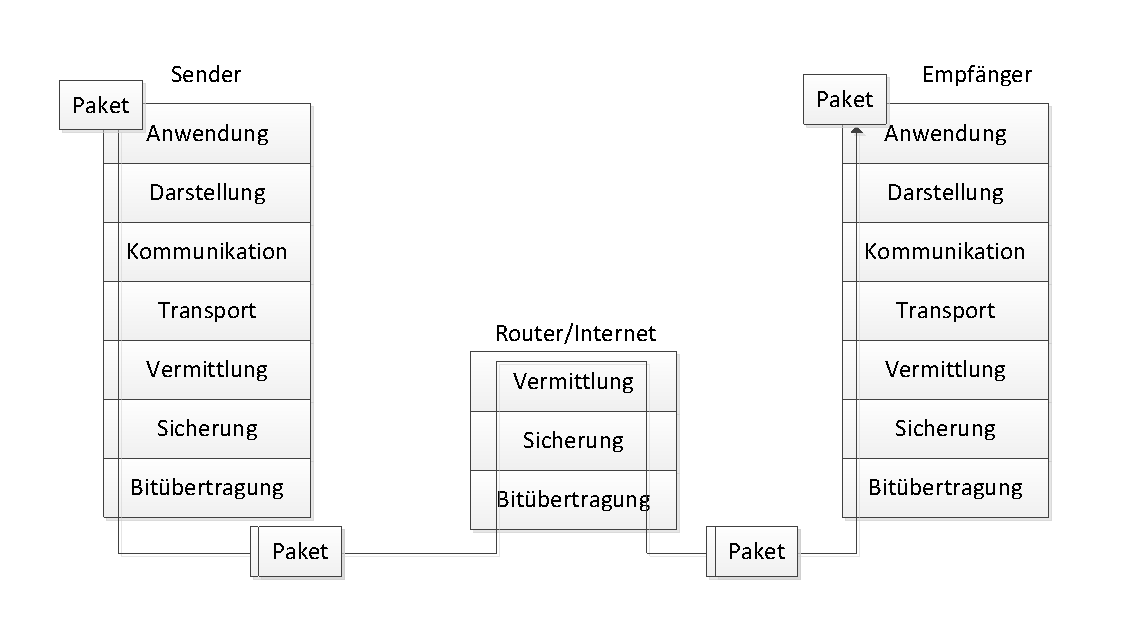
\includegraphics[scale=0.7]{Bilder/OSI.pdf}
  \caption{Kommunikation über das OSI-Schichtenmodell}
  \label{osi}
\end{figure}

\noindent Das OSI-Schichtenmodell wir häufig als Grundlage für den Entwurf neuer Netzwerkprotokolle verwendet. In der Realität finden Kommunikation meist über weniger Schichten statt, wie z.B. das TCP/IP-Referenzmodell.\\

\noindent\textbf{TCP/IP-Referenzmodell}\\
\noindent Das TCP/IP-Referenzmodell basiert auf dem OSI-Modell, fasst jedoch die Aufgaben einiger Schichten zusammen. So wird satt der Bitübertragungs- und Sicherungsschicht eine allgemeine Netzzugangsschicht, und aus Kommunikations-, Darstellungs-, und Anwendungsschicht eine allgemeine Anwendungsschicht. Die Vermittlungs-, und Transportschicht werden beibehalten. \\

\subsection{Netzwerkprotokolle}
Netzwerkprotokolle besitzen je nach Zweck und Netzwerkschicht verschieden Merkmale und Funktionen. Viele Netzwerkprotokolle hängen von der obersten Schicht bis zur Untersten einen eigenen Protokoll Header an. Dieser besitzt wichtige Merkmale zum Transport der darauf folgenden Daten. Einige der wichtigsten Protokolle und deren Header Funktionen werden in diesem Kapitel genauer betrachtet:\\
\\
\begin{itemize}
\item IP: Das Internet Protocol ist ein sehr weit verbreitetes Netzwerkprotokolle welches die Grundlagen des Internet darstellt. Es befindet sich in der Vermittlungsschicht des OSI-Schichtenmodells und ist somit für die Vermittlung über IP-Adressen zuständig.  
\item TCP: Das Transmission Control Protocol ist ein Netzwerkprotokoll der Transportschicht. Dieses garantiert eine zuverlässige, verbindungsorientierte Transport von Paketen in Computernetzwerken. Es zählt wie das IP-Protokoll zu den Grundlagen des Internets. In diesem Protokoll-Header werden der Quell und Ziel Port genannt, um dem meist zuvor erstellten IP-Paket einen bestimmten Dienst zuzuweisen. Eine TCP-Verbindung erfolgt immer über eine vorgegebene Startsequenz. Diese wird 3-Way-Handshake genannt und wir in Abb. \ref{3way} dargestellt. Dabei werden die Control-Flag-Bits im Header jeweils geändert. 

\begin{figure}[h]
    \centering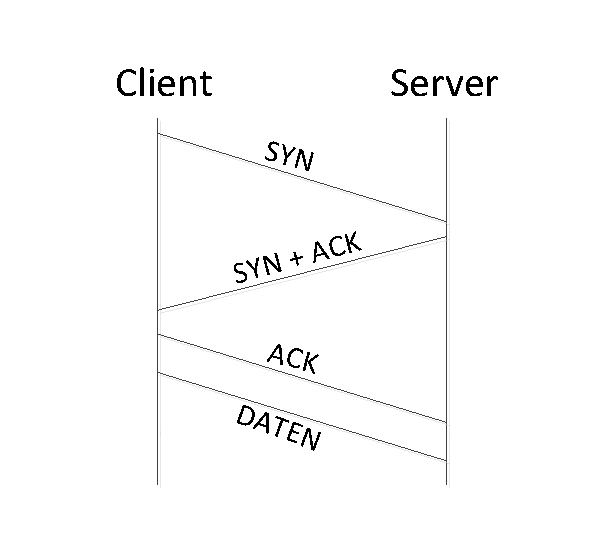
\includegraphics[scale=0.7]{Bilder/3way.pdf}
  \caption{Drei-Wege-Handshake mit TCP}
  \label{3way}
\end{figure}

Nach dem Aufbau der Verbindung können Daten gesendet werden.

\item UDP: Beim User Datagram Protocl handelt es sich um ein verbindungsloses Transportprotokoll. Wie bei TCP befindet sich in seinem Header Ziel- und Quell-Port, jedoch erfolgt kein Verbindungsaufbau. Außerdem wird nicht überprüft, ob alle Pakete tatsächlich beim Benutzer ankommen. 
\item HTTP/HTTPS:Das Hyper Text Transfer Protocol wird von Web-Servern verwendet, um deren Webseiten an den Benutzer zu senden. Diese Protokoll befindet sich bereits in der Anwenderschicht, und baut auf einer TCP/IP Verbindung auf.
\item SSH: Das Secure Shell Protokoll ist ein Netzwerkprotokoll, welches sich ebenfalls auf der Anwenderschicht befindet. Es öffnet eine verschlüsselte Verbindung auf einen entfernten Server, um die Kommandozeile dessen lokal zur Verfügung zu stellen. 
\item FTP: Das File Transfer Protocol wird zur Übertragung von Daten allgemein verwendet. Das Anwendungsprotokoll wird verwendet um vom Server Daten herunter- oder hochzuladen. 
\end{itemize}

\noindent Die Protokolle die in den jeweiligen Schichten angewendet werden, sind oft Angriffsziel vieler Hacker. Diese können über bewusste Manipulation so abgeändert werden, dass das System oft unerwartet reagiert. Einige mögliche Angriffsszenarien werden im folgenden Kapitel betrachtet. 

\newpage

\chapter{Tools und Anwendungen}
In diesem Kapitel werde die von Honeypots und Honeynets verwendeten Tools zum Sammeln von Daten und der Datenaufbereitung genauer betrachtet.

\section{Honeypot und Honeynet Tools}
Snort
Snort\_inline
Hflow2(Gen3)
Tcpdump
Sebek
\\
\subsection{Sebek}
\subsection{Intrusion Detection System}
In Netzwerken werden Intrusion Detection Systeme zur Überwachung und Erkennung von Unregelmäßigkeiten eingesetzt. Im Gegensatz zu einer Firewall, welche erkennbar vor einer DMZ eingesetzt wird, arbeiten IDS im Verborgenen ohne aktiv in das Geschehen einzuschreiten. 
Um den vielfältigen Aufgaben gerecht zu werden, besteht ein IDS aus folgenden vier Modulen:
\begin{itemize}							% Beginn der Aufzählungsumgebung
\item{\textbf{Collection (Sammeln)}} 
\\Für das Sammeln aller relevanten Daten ist das Collection Modul zuständig. Hierbei können zwei verschiedene Vorgehensweisen unterschieden werden. Zum einen gibt es die Host-basierten IDS und zum anderen Netzwerk-basierte Systeme. Soll ein ganzes Netzwerk überwacht werden, eignet sich ein Host basiertes IDS nicht, da hierfür auf jedem Host einzeln ein IDS installiert werden muss. Sinnvoller wäre hier eine Überwachung des Netzwerk-Traffics. Umgesetzt wird das durch sogenannte Sensoren die im Netz eingebunden werden und dort die Daten abgreifen. Möglich ist das an einem Switchport der als Monitoring-Port konfiguriert wird. Ein solches Vorgehen wird Netzwerk basiertes Intrusion Detection System genannt. 
\item{\textbf{Detection (Erkennen)}} 
\\Um einen Angriff erkennen zu können gibt es diverse Möglichkeiten. Ein Pattern basiertes System vergleicht die gesammelten Daten mit gespeicherten Pattern, welche aus bekannten Gefahren bestehen. Sobald es Übereinstimmungen gibt handelt es sich meist um einen Angriff. Nachteil hierbei ist, dass regelmäßig Updates eingespielt werden müssen, ähnlich wie es bei einem Anti-Viren Programm ist.

Eine Alternative ist ein Anomalie-Detection-System. Bei diesem Vorgehen wird in einer ersten Phase der Netzwerk-Verkehr mitgeschnitten und gespeichert. Aus den gesammelten Daten leitet das System einen \glqq normalen\grqq Zustand ab. In der zweiten Phase vergleicht das System den aktuellen Traffic mit dem von ihm als \glqq zulässigen\grqq gespeicherten Traffic und sucht nach Abweichungen. Vorteil hierbei ist, dass auch nicht bekannte Angriffe erkannt werden können.
\item{\textbf{Analyse (Analysieren)}} 
\\Das Analyse Modul bereitet die Ergebnisse des vorherigen Moduls grafisch auf und in gibt Statistiken über die ausgewerteten Daten aus. 
\item{\textbf{Response (Reaktion)}} 
\\Häufig greift ein IDS nicht aktiv in den Netzwerk-Traffic ein um weiterhin unerkannt zu bleiben. Dennoch sollte ein Intrusion Detection System handeln wenn ein verdächtiges Verhalten entdeckt wird. Um das Vorgehen des möglichen Angriffs besser rekonstruieren zu können sollten die verdächtigen Aktivitäten mitgeloggt werden. Bei möglichen kritischen Problemen können unter Umständen auch Alarme, in Form von SMS oder E-Mail an den Administrator, erzeugt werden.
\end{itemize}
Bei genauer Betrachtung der Arbeitsweise zeigt sich, warum ein Honeypot oft auch als Teil eines IDS angesehen wird. Sowohl ein Host basiertes, als auch ein Netzwerk basiertes IDS bietet die Möglichkeit einen Honeypot zu überwachen und das Verhalten eines Angreifers zu dokumentieren. Um Handlungen auf dem Honeypot nachvollziehen zu können eignet sich jedoch ein Host basiertes System deutlich besser, da hier auch die Aktionen auf dem Host geloggt werden können. Die Überwachung des Honeypots gestaltet sich deutlich einfacher als die eines normalen Systems. Denn auch hier gilt jeder Zugriff auf den Honeypot als potentieller Angriff. Somit muss das IDS nicht entscheiden, nach welchen Mustern Angriffe gedeutet werden. 

Abschließend kann festgehalten werden: Für diese Arbeit dient ein IDS aus Sicht eines Honeypots zur Aufzeichnung und Auswertung der Angriffe, sowie zur Alarmierung. Dies schließt ausdrücklich nicht die Ansicht aus, dass ein Honeypot Teil eines IDS sein kann. In diesem Fall kommt es nur auf den Blickwinkel an, aus dem das Thema betrachtet wird.
\section{Honeypot Software}
\subsection{Honeyd}
Honeyd ist ein von Niels Provos entwickelter Honeypot Deamon, der verschiedene virtuelle Host Systeme wie Workstations oder Netzwerkgeräte emulieren kann. Somit ist es möglich, eine komplette Netzstruktur zu emulieren. Die Open Source Sofware wird unter GPL veröffentlicht, und ist somit ohne Lizenzkosten benutzbar. Die aktuelle Version 1.5c wurde am 27.05.2007 veröffentlicht. Über die Benutzung von Konfigurationsdateien kann eine vielzahl von Betriebssystemen gewählt werden. Dabei werden s.g. Templates erstellt, für die zuerst eine Identität gewählt werden muss. Danach können verschiedene Parameter das simulierte Verhalten des virtuellen Clients festgelegt werden. Dazu gehören z.B. das eine emulierte Bandbreite des Übertragungskanals, Default-Aktionen verschiedener Ports und die zu aktivierenden Scripts beim Zugriff auf verschiedenen Ports. Zuletzt wird dem Template die gewünschte IP zugewiesen. In einer Honeyd Konfigurationsdatei können mehrere Clients eingetragen werden werden. Ein minimales Beispiel einer Honeyd-Konfigurationsdatei befindet sich in Abb. \ref{honeydConf}. Die Skripte, die bei einem versuchten Zugriff auf einem Port gestartet werden sollen können beliebig erstellt oder manipuliert werden. 
\\
\begin{figure}[ht]
    \centering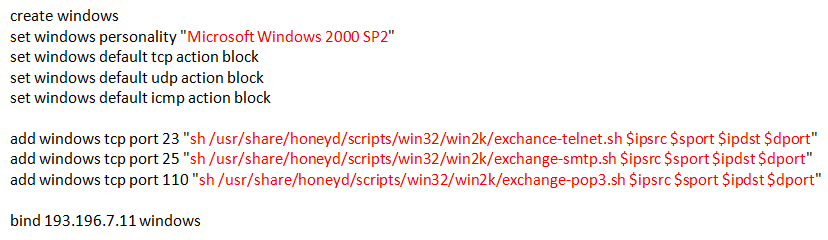
\includegraphics[scale=0.7]{Bilder/HoneydConf.png}
  \caption{Beispielkonfiguration einer Honeyd Config-Datei}
  \label{honeydConf}
\end{figure}

Honeyd wird unter Unix Systemen in der Kommandozeile ausgeführt. Dabei stellt das Programm verschiedene Konfigurationsmöglichkeiten zur Verfügung. Über den Parameter honeyd -d wird das Programm nicht als Deamon gestartet. So kann man in der Konsole nach starten des Programmes die erfolgten Zugriffe beobachten. Diese möglicherweise versuchten Angriffe (je nach Netz werden auch alle Pakete die an die Broadcast Adresse gesendet werden empfangen) müssen danach analysiert werden. Um ein möglichst leicht auswertbares Ergebnis zu erhalten kann eine feste Angabe des abzuhörenden Netzbereichs sowie die Erstellung einer Log-Datei erfolgen. Der folgende Befehl kann so auf das zuvor genannte Beispiel angewandt werden:\\
\\
\noindent\emph{honeyd -f honeyd.conf 193.196.7.11 -l honeyd.log}\\
\\
Hierbei werden nur die Pakete die für die Zieladresse 193.196.7.11 bestimmt sind für eine Auswertung in Betracht gezogen. Die erfolgten Zugriffe werden in der Datei honeyd.log gespeichert.
Die Log-Dateien speichern folgende Datensätze: \\
\\
\noindent\emph{2014-02-22-15:50:59.5296 tcp(6) S 109.193.95.133 21473 193.196.7.11 23 [Windows 2000 RFC1323]}\\
\\
Zunächst wird der Zeitpunkt des Angriffes festgestellt. Danach ob der Zugriff über TCP, UDP oder ICMP stattgefunden hat. Das S kennzeichnet den Start einer Verbindung. Bei UDP oder Paketen, die das Ende einer Verbindung kennzeichnen befindet sich an dieser Stelle ein E. Die nächsten beiden Werte sind die Quelle und Ziel IP-Adressen mit dem dazugehörigen Ports. Zuletzt befindet sich ein Versuch über Passive Fingerprinting das Betriebssystem des Angreifers zu erraten. 
Bei diesem Beispiel handelt es sich um einen Versuch über Telnet auf den Honeypot zuzugreifen. Da Honeyd seit 2007 nicht mehr weiterentwickelt wird verwendet es in diesem Beispiel eine veraltete Fingerprint Datenbank und gibt statt des verwendeten Windows 8.1 einen Windows 2000 Rechner an. 
\subsection{Tiny oder Tarpit}
\subsection{Roo}

\subsection{Virtuelle Honeypots}
\section{Anwendungen zur Datenanalyse}

\subsection{Honey View}
\subsection{...}
\newpage

\chapter{Implementierung des Honeypots}

\section{Verwendete Software}
\section{Honeyd Implementierung}
In diesem Kapitel wird genauer auf die konkrete Erstellung des Honeyd Honeypots mit allen Problemstellungen eingegangen. 
\subsection{Installation}
Die zum Zeitpunkt der Studienarbeit aktuelle Version von Honeyd ist 1.5c. Diese Version wurde am 27.05.2007 veröffentlicht und ist demnach recht veraltet. Die Webseite von Niels Provos zu diesem Projekt wurde zuletzt am 15.07.2008 bearbeitet, demnach davon ausgegangen werden kann das er das Projekt nicht mehr weiter verfolgt. Honeyd ist jedoch mit Einschränkungen auf den meisten Unixartigen System lauffähig.
Vor der Installation des eigentlichen Honeyd Deamons müssen einige Abhängigkeiten installiert werden:\\
\\
\noindent\textbf{libdnet:}\\
libdnet ist eine Programmbibliothek die Zugriff auf low-level Netzwerkroutinen gewährt. Dazu gehören z.B. Netzwerkadressmanipulation, Netzwerkfirewallmanipulation, Netzwerinterfacezugriff, IP-Tunneling und Zugriff auf einzelne IP-Pakete.\\\\
\noindent\textbf{libevent:}\\
libenvent ist eine Programmbibliothek, die eine asynchrone Benachrichtigungsfunktion besitzt, die bei bestimmten Events oder nach vordefinierten Timeouts ausgelöst werden kann.\\\\
\noindent\textbf{libpcap:}\\
libpcpa ist eine freie Programmierschnittstelle zur Überwachung des Netzverkehrs. Viele Netzwerkanalysetools greifen auf die Funktion von pcpa (packet capture) Bibliotheken zurück. libpcap ist eine Programmbibliothek für unixartige System, WinPcap besitzt für Windows Betriebssysteme die selbe Funktion. Wireshark, Snort und Nmap greifen z.B. auf die selbe Schnittstelle zurück.\\
\\
Für erweiterte Funktionen wurde das Paket Honeyd-commmons ebenfalls heruntergeladen. In diesem befinden sich zusätzliche Dokumentationen und Skripte für die Nachahmung verschiedener Services. Nach der Installation aller notwendiger Pakete müssen Konfigurationen für den Deamon erstellt werden.
\subsection{Konfiguration}
\subsection{Datenanalyse}
\section{Kommerzielle Implementierung}

\subsection{Installation}
\subsection{Konfiguration}
\subsection{Datenanalyse}
\section{Open Source Implementierung}

\subsection{Installation}
\subsection{Konfiguration}
\subsection{Datenanalyse}
\newpage

\chapter{Auswertung der gesammelten Daten}
\newpage

\chapter{Fazit}
\newpage

\section*{Anhang}

				% Anhang Einbinden
%%%%%%%%%%%%%%%%%%%%%%%%%%%%%%%%%% Literaturverzeichnis %%%%%%%%%%%%%%%%%%%%%%%%%%%%%%%%%%%%%%%%%%%%%%%%%%%%%%%%%%%%%%%%%%%%%%%%%%%%%%%%%%%%%%%%%%%%%%%%%%%%%%%%%%%%%%%%%%
\addcontentsline{toc}{chapter}{Literaturverzeichnis}
\bibliographystyle{gerabbrv}				% Zitierformat (deutsch für Großschreibung) [Häufigkeit] im Text
\bibliography{Literaturverzeichnis}			% Pfad des Literaturverzeichnisses

\end{document}  %%%%%%%%%%%%%%%%%%%%%%%%%%%%%%%%%%%%%%%%%%%%%%%%%%%%%%%%%%%%%%%%%%%%%%%%%%%%%%%%%%%%%%%%%%%%%%%%%%%%%%%%%%%%%%%%%%%%%%%%%%%%%%%%%%%%%%%%%%%%%%%%%%%%%%%%%%
